\section{Introduction}

\begin{frame}
\frametitle{Motivación}
\framesubtitle{Objetivos}

\begin{itemize}
\item{Formalizar la semántica de un lenguaje imperativo con procedimientos, arreglos y apuntadores}
\item{Proveer un mecanismo de traducción a un lenguaje imperativo real}
\end{itemize}

\pause

Actividades de este proyecto
\begin{itemize}
\item{Formalizar la semántica de un lenguaje imperativo llamado Chloe}
\item{Escribir un interpretador para el lenguaje}
\item{Demostraciones de determinismo y correctitud}
\item{Escribir un traductor a código C}
\item{\textit{Testing}}
\end{itemize}

\end{frame}

\begin{frame}
\frametitle{Motivación}
\framesubtitle{El lenguaje de programación C}

\pause

Lenguaje C:

\pause

\begin{itemize}
\item{Cercanía  a la máquina y bajo \textit{overhead} permiten eficiencia.}
\pause
\item{Utilizado para sistemas operativos, aplicaciones de sistemas embebidos, compiladores, librerías e interpretadores.}
\pause
\end{itemize}

Desventaja?
\pause
\begin{itemize}
\item{Parte de la semántica se define en lenguaje natural, lo cual la hace vulnerable a ambigüedades.}
\end{itemize}

\end{frame}


\begin{comment}
\begin{frame}
\frametitle{Motivación}
\framesubtitle{Objetivos del trabajo}

\pause
\begin{itemize}
\item{Formalizar la semántica operacional de pasos cortos de un lenguaje imperativo que represente un subconjunto especializado y determinístico de la semántica de C.}
\pause
\item{Escribir un interpretador dentro del ambiente de Isabelle/HOL y demostrar su correctitud.}
\pause
\item{Generar código C a partir de programas escritos en la semántica formal.}
\pause
\item{Crear un ambiente de pruebas y una batería de pruebas que incrementen la confianza en el proceso de generación de código.}
\end{itemize}

\end{frame}
\end{comment}


\begin{frame}
\frametitle{Chloe}
\framesubtitle{Un lenguaje imperativo, subconjunto de C}

\begin{columns}[t]
\column{.45\textwidth}
\begin{block}{Características actuales:}
\pause
\begin{itemize}
\item{Variables}
\pause
\item{Arreglos}
\pause
\item{Aritmética de apuntadores}
\pause
\item{Ciclos}
\pause
\item{Condicionales}
\pause
\item{Funciones}
\pause
\item{Memoria dinámica}
\pause
\end{itemize}
\end{block}
\column{.45\textwidth}
\begin{block}{Extensiones a futuro:}
\begin{itemize}
\pause
\item{Sistema de tipos estático correcto y completo}
\pause
\item{Concurrencia}
\pause
\item{Operaciones I/O}
\pause
\item{Goto}
\pause
\item{Etiquetas}
\pause
\item{Instrucciones break y continue}
\end{itemize}
\pause
\end{block}
\end{columns}

\end{frame}


\begin{frame}
\frametitle{Semántica}


Existen tres enfoques principales:

\bigskip

\only<1>{
Operacional:

\bigskip
Describe el significado de un programa en función del efecto que tiene cada construcción del lenguaje sobre un estado suponiendo una máquina abstracta.
  \begin{itemize}
    \item{Pasos largos}
    \item{Pasos cortos}
  \end{itemize}
}
\only<2>{
Denotacional:

\bigskip
Describe el significado de un programa en función de una estructura mátemática o dominio que represente el estado de un programa y el comportamiento de las construcciones en el lenguaje corresponde a una componente de la estructura matemática.
}

\only<3>{
Axiomática:

\bigskip
Describe el significado de las construcciones de lenguaje mediante predicados lógicos, de modo que el efecto de cada construcción es un par de predicados que describen el estado antes y despues de ejecutar la instrucción.
}

\end{frame}

\begin{frame}
\frametitle{Isabelle/HOL}

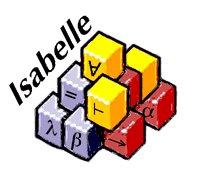
\includegraphics[scale=0.5]{images/isabelle.png}

\begin{itemize}
\item{Isabelle/HOL es un demostrador interactivo de teoremas escrito en ML.}
\item{Desarrollado por Larry Paulson y Tobias Nipkow.}
\item{Utiliza el lenguaje HOL para realizar las pruebas.}
\item{Permite hacer definiciones y demostrar propiedades acerca de las mismas.}
\item{Se usa la máquina para asistir en las demostraciones}
\end{itemize}

\end{frame}

\begin{frame}
\frametitle{Ejemplo de una prueba en Isabelle/HOL}

\begin{semiverbatim}
datatype \textit{nat} = 0 | Suc \textit{nat}


fun add :: ``nat => nat => nat'' where

Base: ``add 0 n = n'' |

Rec: ``add (Suc m) n = Suc (add m n)''
\end{semiverbatim}

\end{frame}

\begin{frame}
\frametitle{Ejemplo de una prueba en Isabelle/HOL}

\begin{columns}[t]
\column{.45\textwidth}
\begin{semiverbatim}
\only<1-8>{
lemma add\_right:

``add m 0 = m''

proof(induction)}

\only<2-8>{
\alert<2>{show ``add 0 0 = 0''}

}
\only<3-8>{
  \alert<3>{using Base}

}
\only<4-8>{
  \alert<4>{by simp}

}

\only<5-8>{
\alert<5>{fix x

assume IH: ``add m 0 = m''
}}
\only<6-8>{
\alert<6>{show ``add (Suc m) 0 = Suc m''}

}
\only<7-8>{
  \alert<7>{using Rec and IH}

}
\only<8>{
  \alert<8>{by simp}

qed}

\only<9->{
lemma add\_right:

``add m 0 = m''


apply induction

apply auto

done}


\end{semiverbatim}
\column{.45\textwidth}
\begin{block}{Output de Isabelle}
\begin{semiverbatim}
\only<1>{
goal (2 subgoals):

1. add 0 0 = 0

2. $\bigwedge$ x. add x 0 = x $\Longrightarrow$
add (Suc x) 0 = Suc x

}
\only<2>{
goal (1 subgoal):

\alert<2>{1. add 0 0 = 0}

}
\only<3>{
\alert<3>{using this:

  add 0 ?n = ?n}


goal (1 subgoal):

1. add 0 0 = 0

}
\only<4>{
goal (1 subgoal):

\alert<4>{1. $\bigwedge$ x. add x 0 = x $\Longrightarrow$
add (Suc x) 0 = Suc x}

}
\only<5>{
\alert<5>{this:

add x 0 = x}

goal (1 subgoal):

1. $\bigwedge$ x. add x 0 = x $\Longrightarrow$
add (Suc x) 0 = Suc x

}
\only<6>{
goal (1 subgoal):

\alert<6>{1. add (Suc x) 0 = Suc x}

}
\only<7>{
\alert<7>{using this:

add (Suc ?m) ?n = Suc (add ?m ?n)

add x 0 = x}


goal (1 subgoal):

1. add (Suc x) 0 = Suc x

}
\only<8-9>{
goal:

\alert<9>{No subgoals!}

}

\end{semiverbatim}
\end{block}
\end{columns}


\end{frame}

\begin{comment}

\end{comment}
